\documentclass{beamer}

\usepackage{hyperref}
\usepackage{graphicx}
\graphicspath{ {images/} }

\usetheme{Madrid}
\usecolortheme{default}
\setbeamertemplate{navigation symbols}{}

\begin{document}

\title{Gamification of Clinical Practice Guidelines}
\author{Ben-Richard Ebbesvik}
\institute{Western Norway University of Applied Sciences \newline University of Bergen}
\date{3rd of April 2019}
\subject{Master thesis}
\frame{\titlepage}


\begin{frame}{Introduction}
\begin{itemize}
	\item The tool will be developed in cooperation with medical doctor and PhD student Job Nyangena Nyameino.
	\item The target group for the tool will primarily be medical students and clinicians located in Norway and Kenya.
	\item A key to making these tools is clinical practice guidelines
\end{itemize}
\begin{block}{Definition}	
	 "Clinical Practice Guidelines are statements that include recommendations intended to optimize patient care that are informed by a systematic review of evidence and an assessment of the benefits and harms of alternative care options." (The Institute of Medicine 2011)
\end{block}
\end{frame}

\begin{frame}{Possible asthma in paediatrics - Norway}
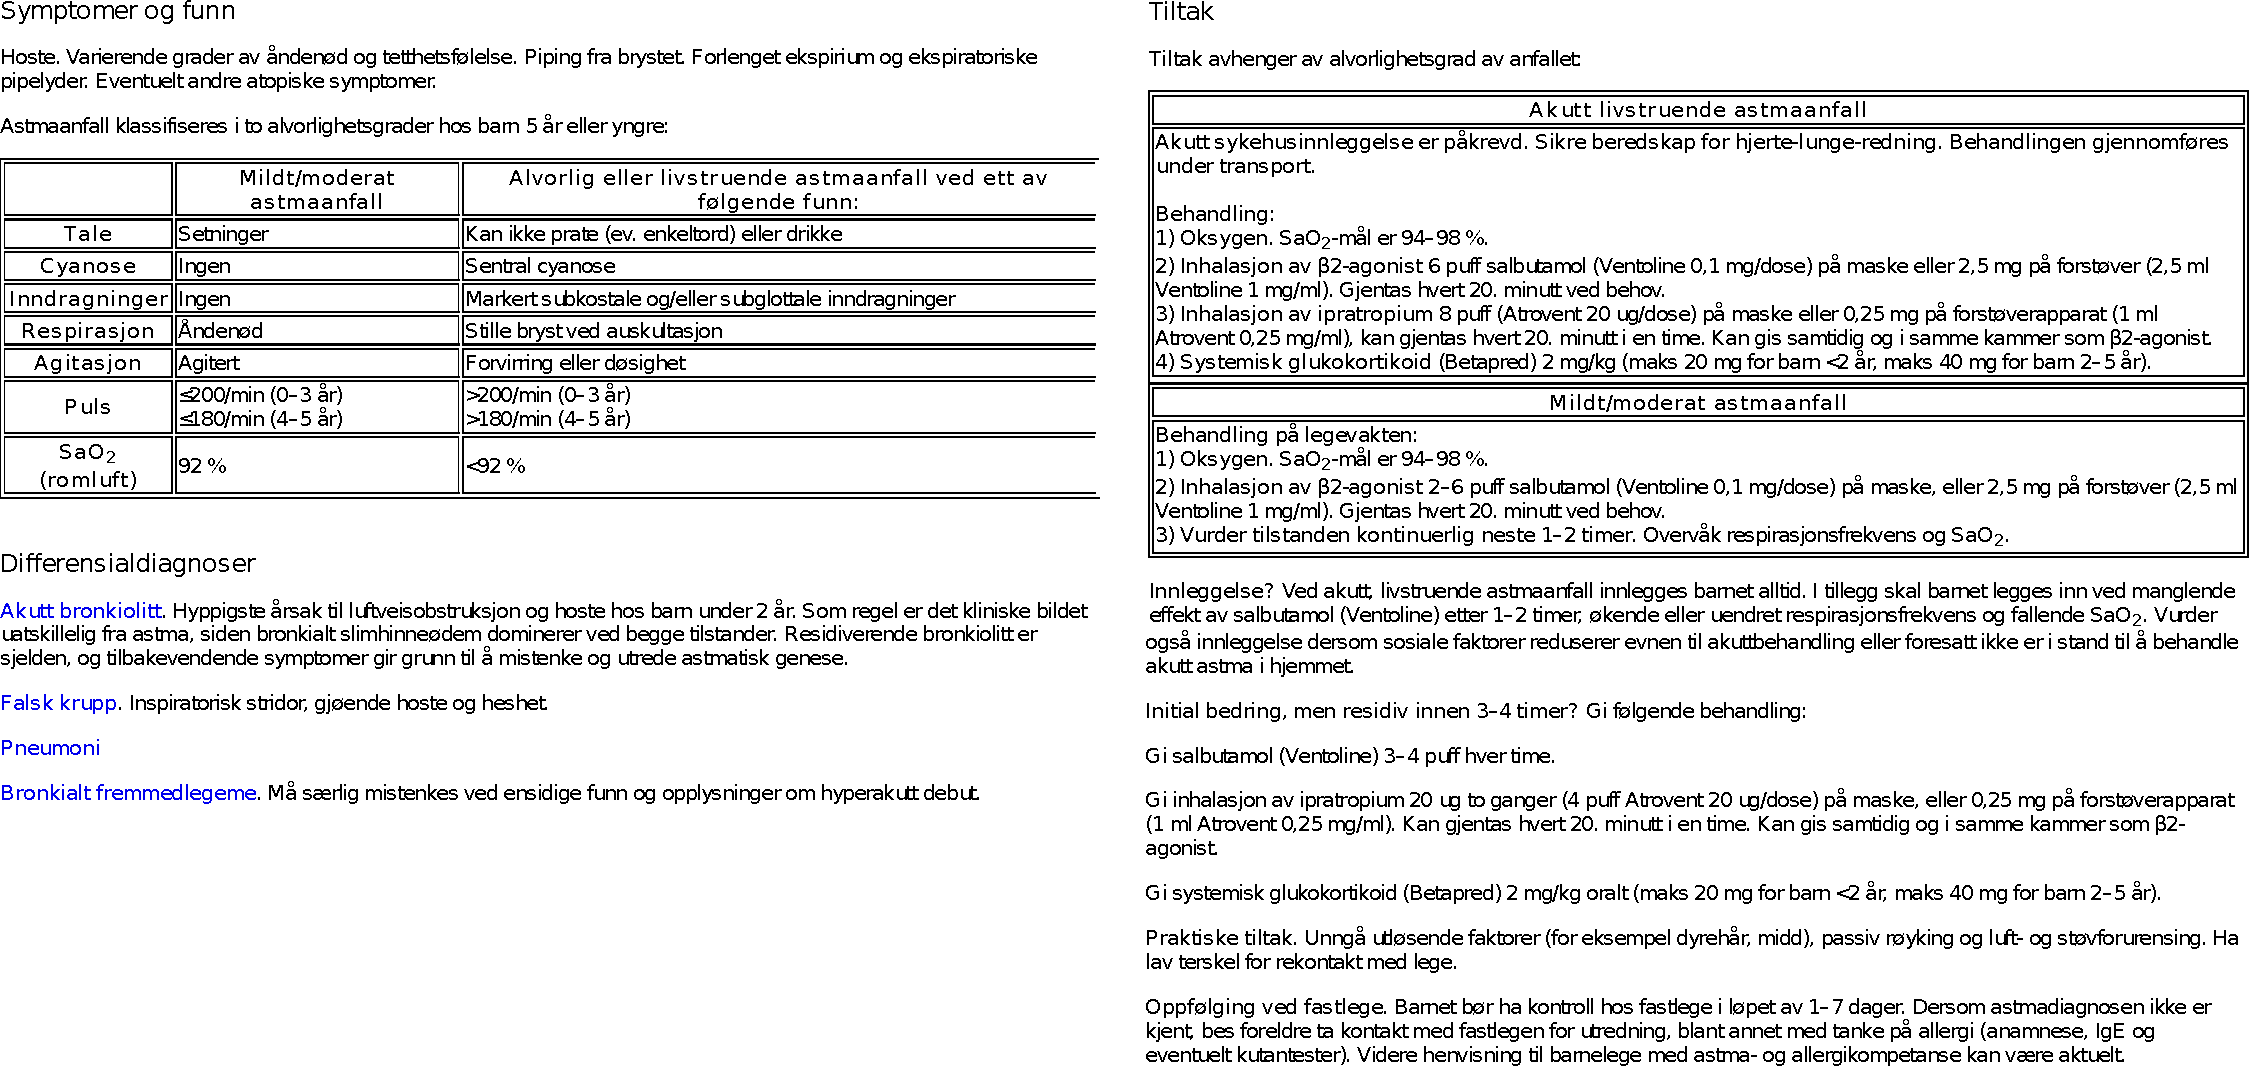
\includegraphics[scale=0.32]{NorwayCPG}
\end{frame}


\begin{frame}{Research questions}
\begin{itemize}
		\item Based on clinical guidelines, can we make a reusable data structure representing respiratory diseases for use in serious games?
		\begin{itemize}
			\item Can we use such a model for generating case based multiple choice questions and answer elements?
			\item Can we use the data model to structure the learning content such that it is adapted to the current knowledge of the individual learner?
		\end{itemize}		
\end{itemize}
\end{frame}


\begin{frame}{Approach}
Design science
\begin{itemize}
	\item Problem: CPGs have proven to have a great potential, but are not used enough.
	\item Design an artefact that will contribute to more use of CPGs.
	\item Evaluation of the artefact will give us more knowledge around the domain and challenges. The research will come from the design. Improve and adjust the artefact accordingly. 
	\item Iterate and increment.
\end{itemize}
\end{frame}

\begin{frame}{Possible asthma in paediatrics - Kenya}
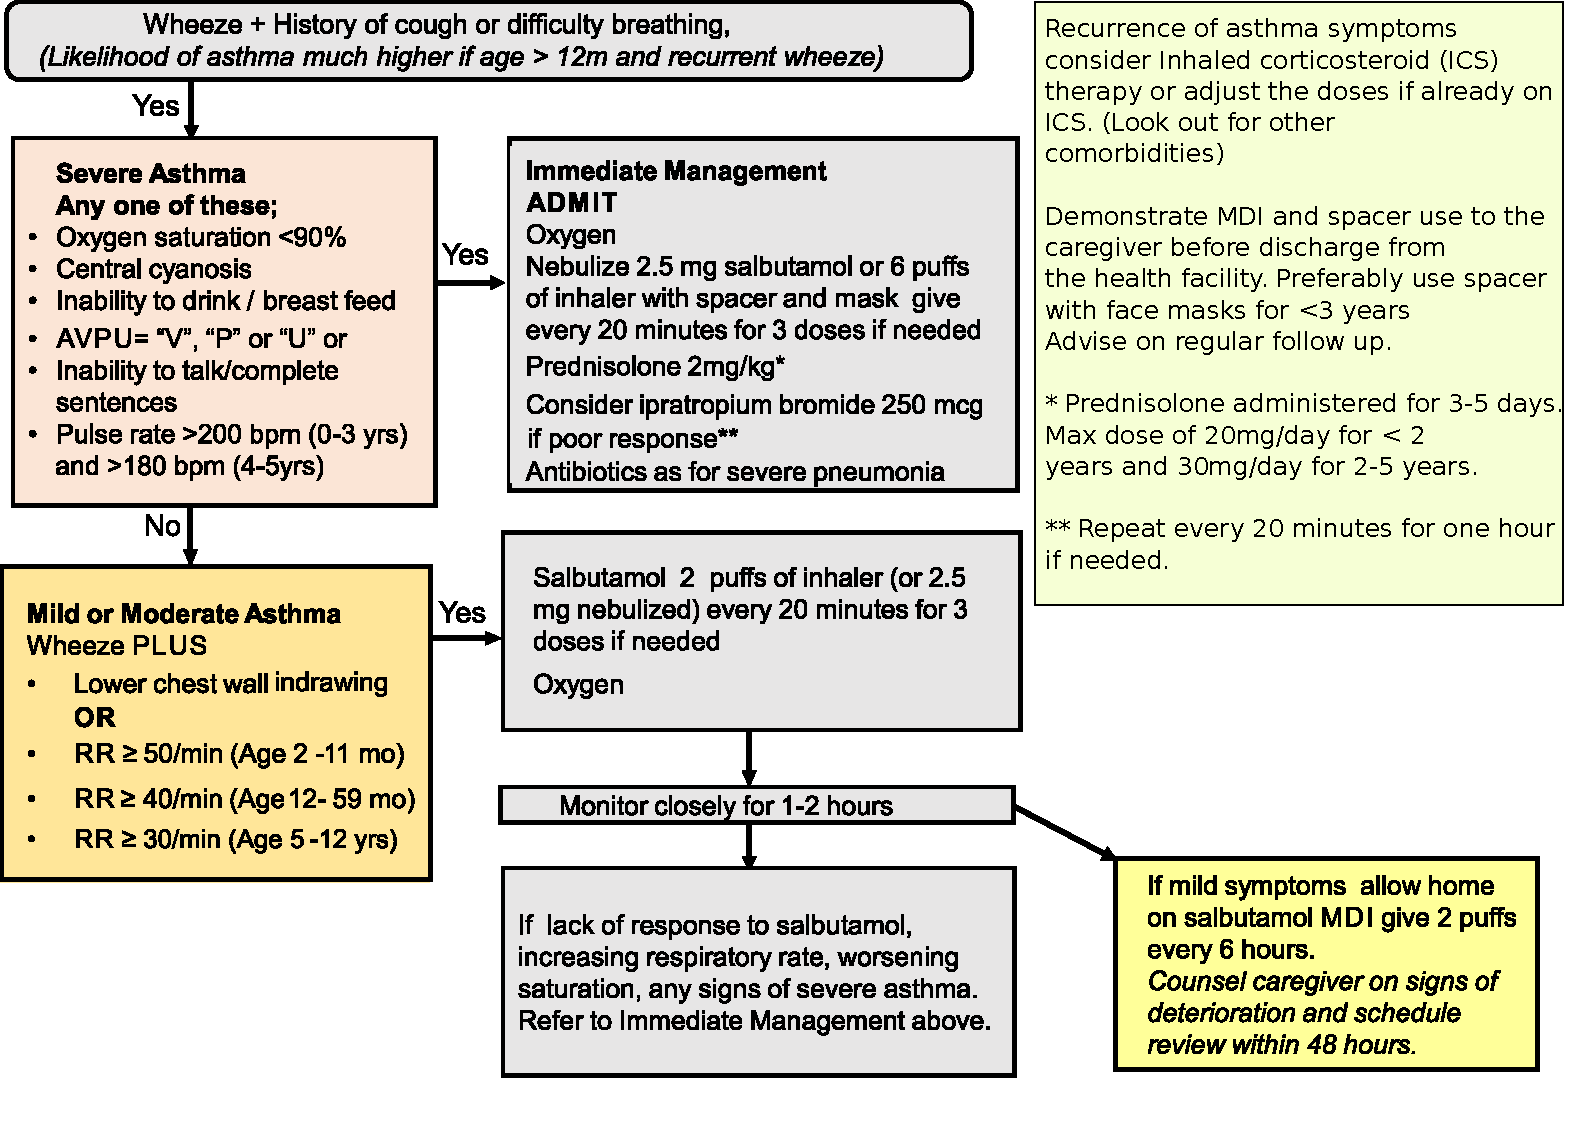
\includegraphics[scale=0.45]{KenyaCPG}
\end{frame}


\begin{frame}{Entity graph}
Show the entity graph here. At least the large and important pieces...
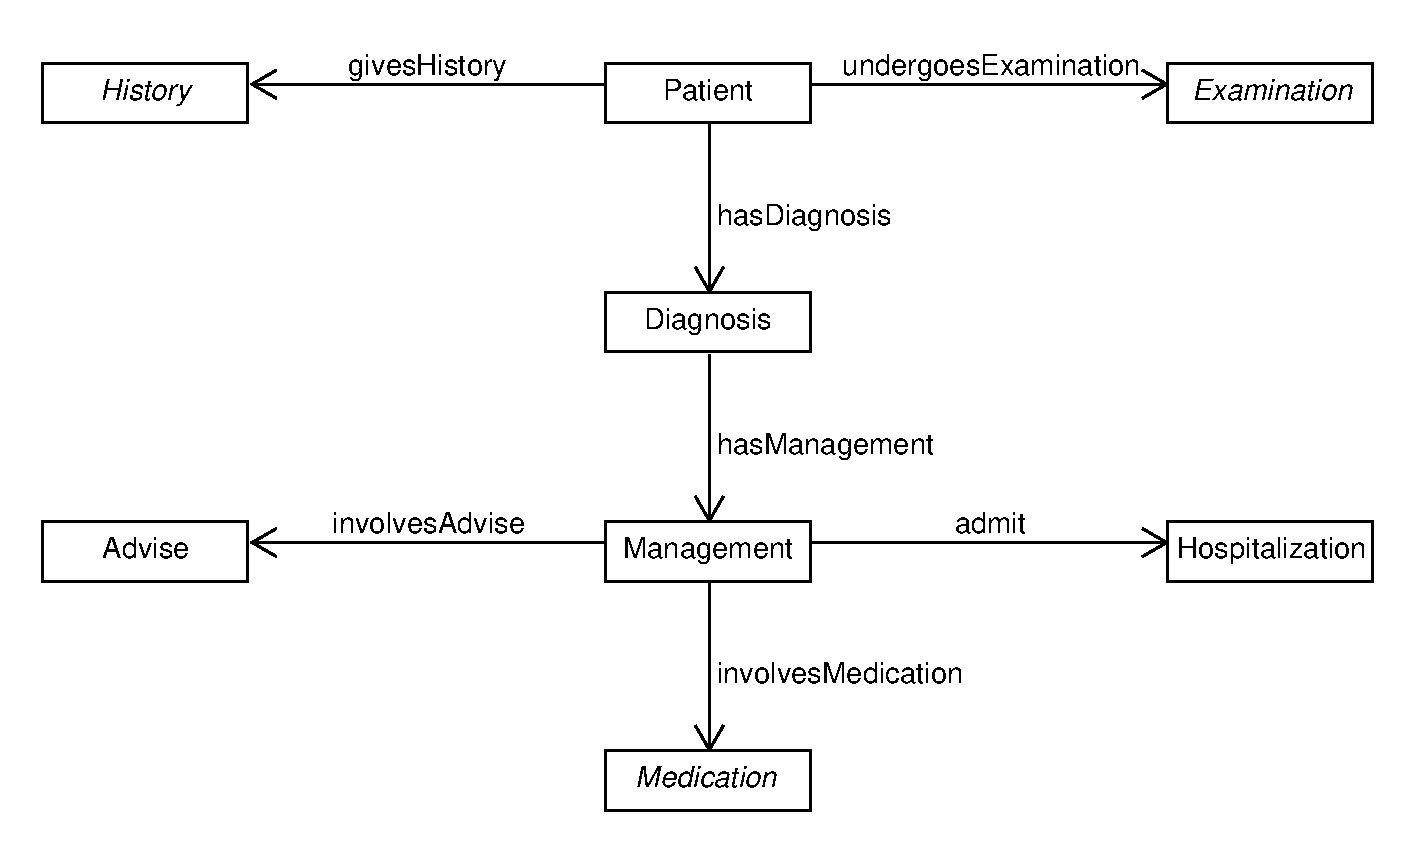
\includegraphics[scale=0.45]{SimpleEntityGraph}
\end{frame}


\begin{frame}[fragile]
\frametitle{Making scenarios, answer keys, distractions}
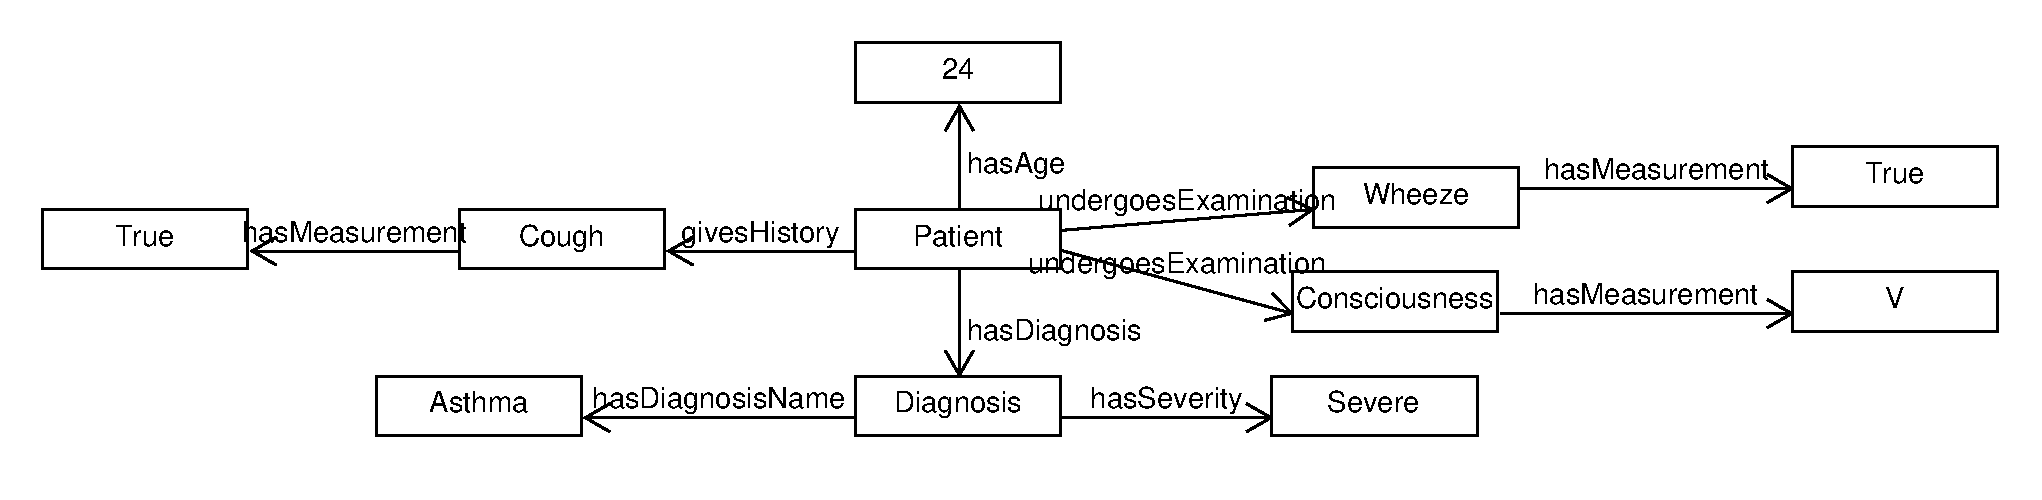
\includegraphics[scale=0.36]{EntityInstanceGraph}
\begin{semiverbatim}
A <\%Patient.hasAge.Age\%> old has arrived at the 
emergency clinic.  
She <\%Patient.givesHistory.Cough\%> 
<\%Patient.undergoesExamination.Wheeze\%>
<\%Patient.undergoesExamination.Consciousness\%>
\end{semiverbatim}
\end{frame}

\begin{frame}[fragile]
\frametitle{Making scenarios}
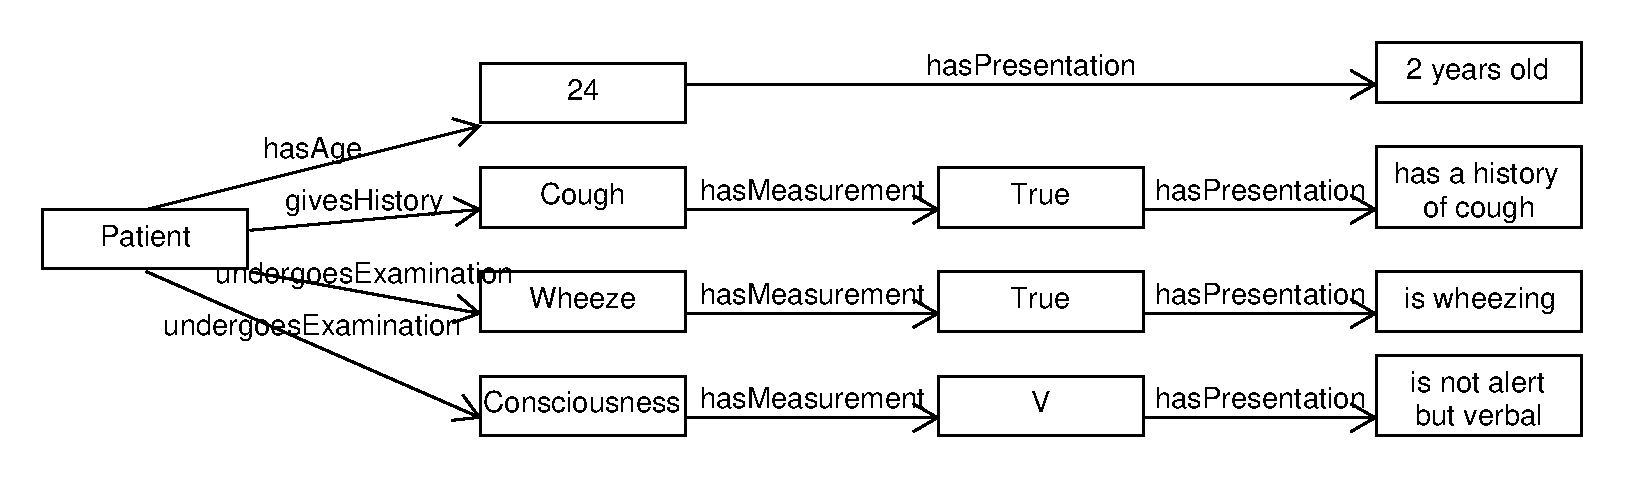
\includegraphics[scale=0.45]{PresentationEntityGraph}
\begin{semiverbatim}
	A 2 year old has arrived at the 
	emergency clinic.  
	She has a history of cough, 
	is wheezing
	and is not alert but verbal.
\end{semiverbatim}
\end{frame}

\begin{frame}{Dynamic Content Management}
\end{frame}


\begin{frame}{Demonstration}
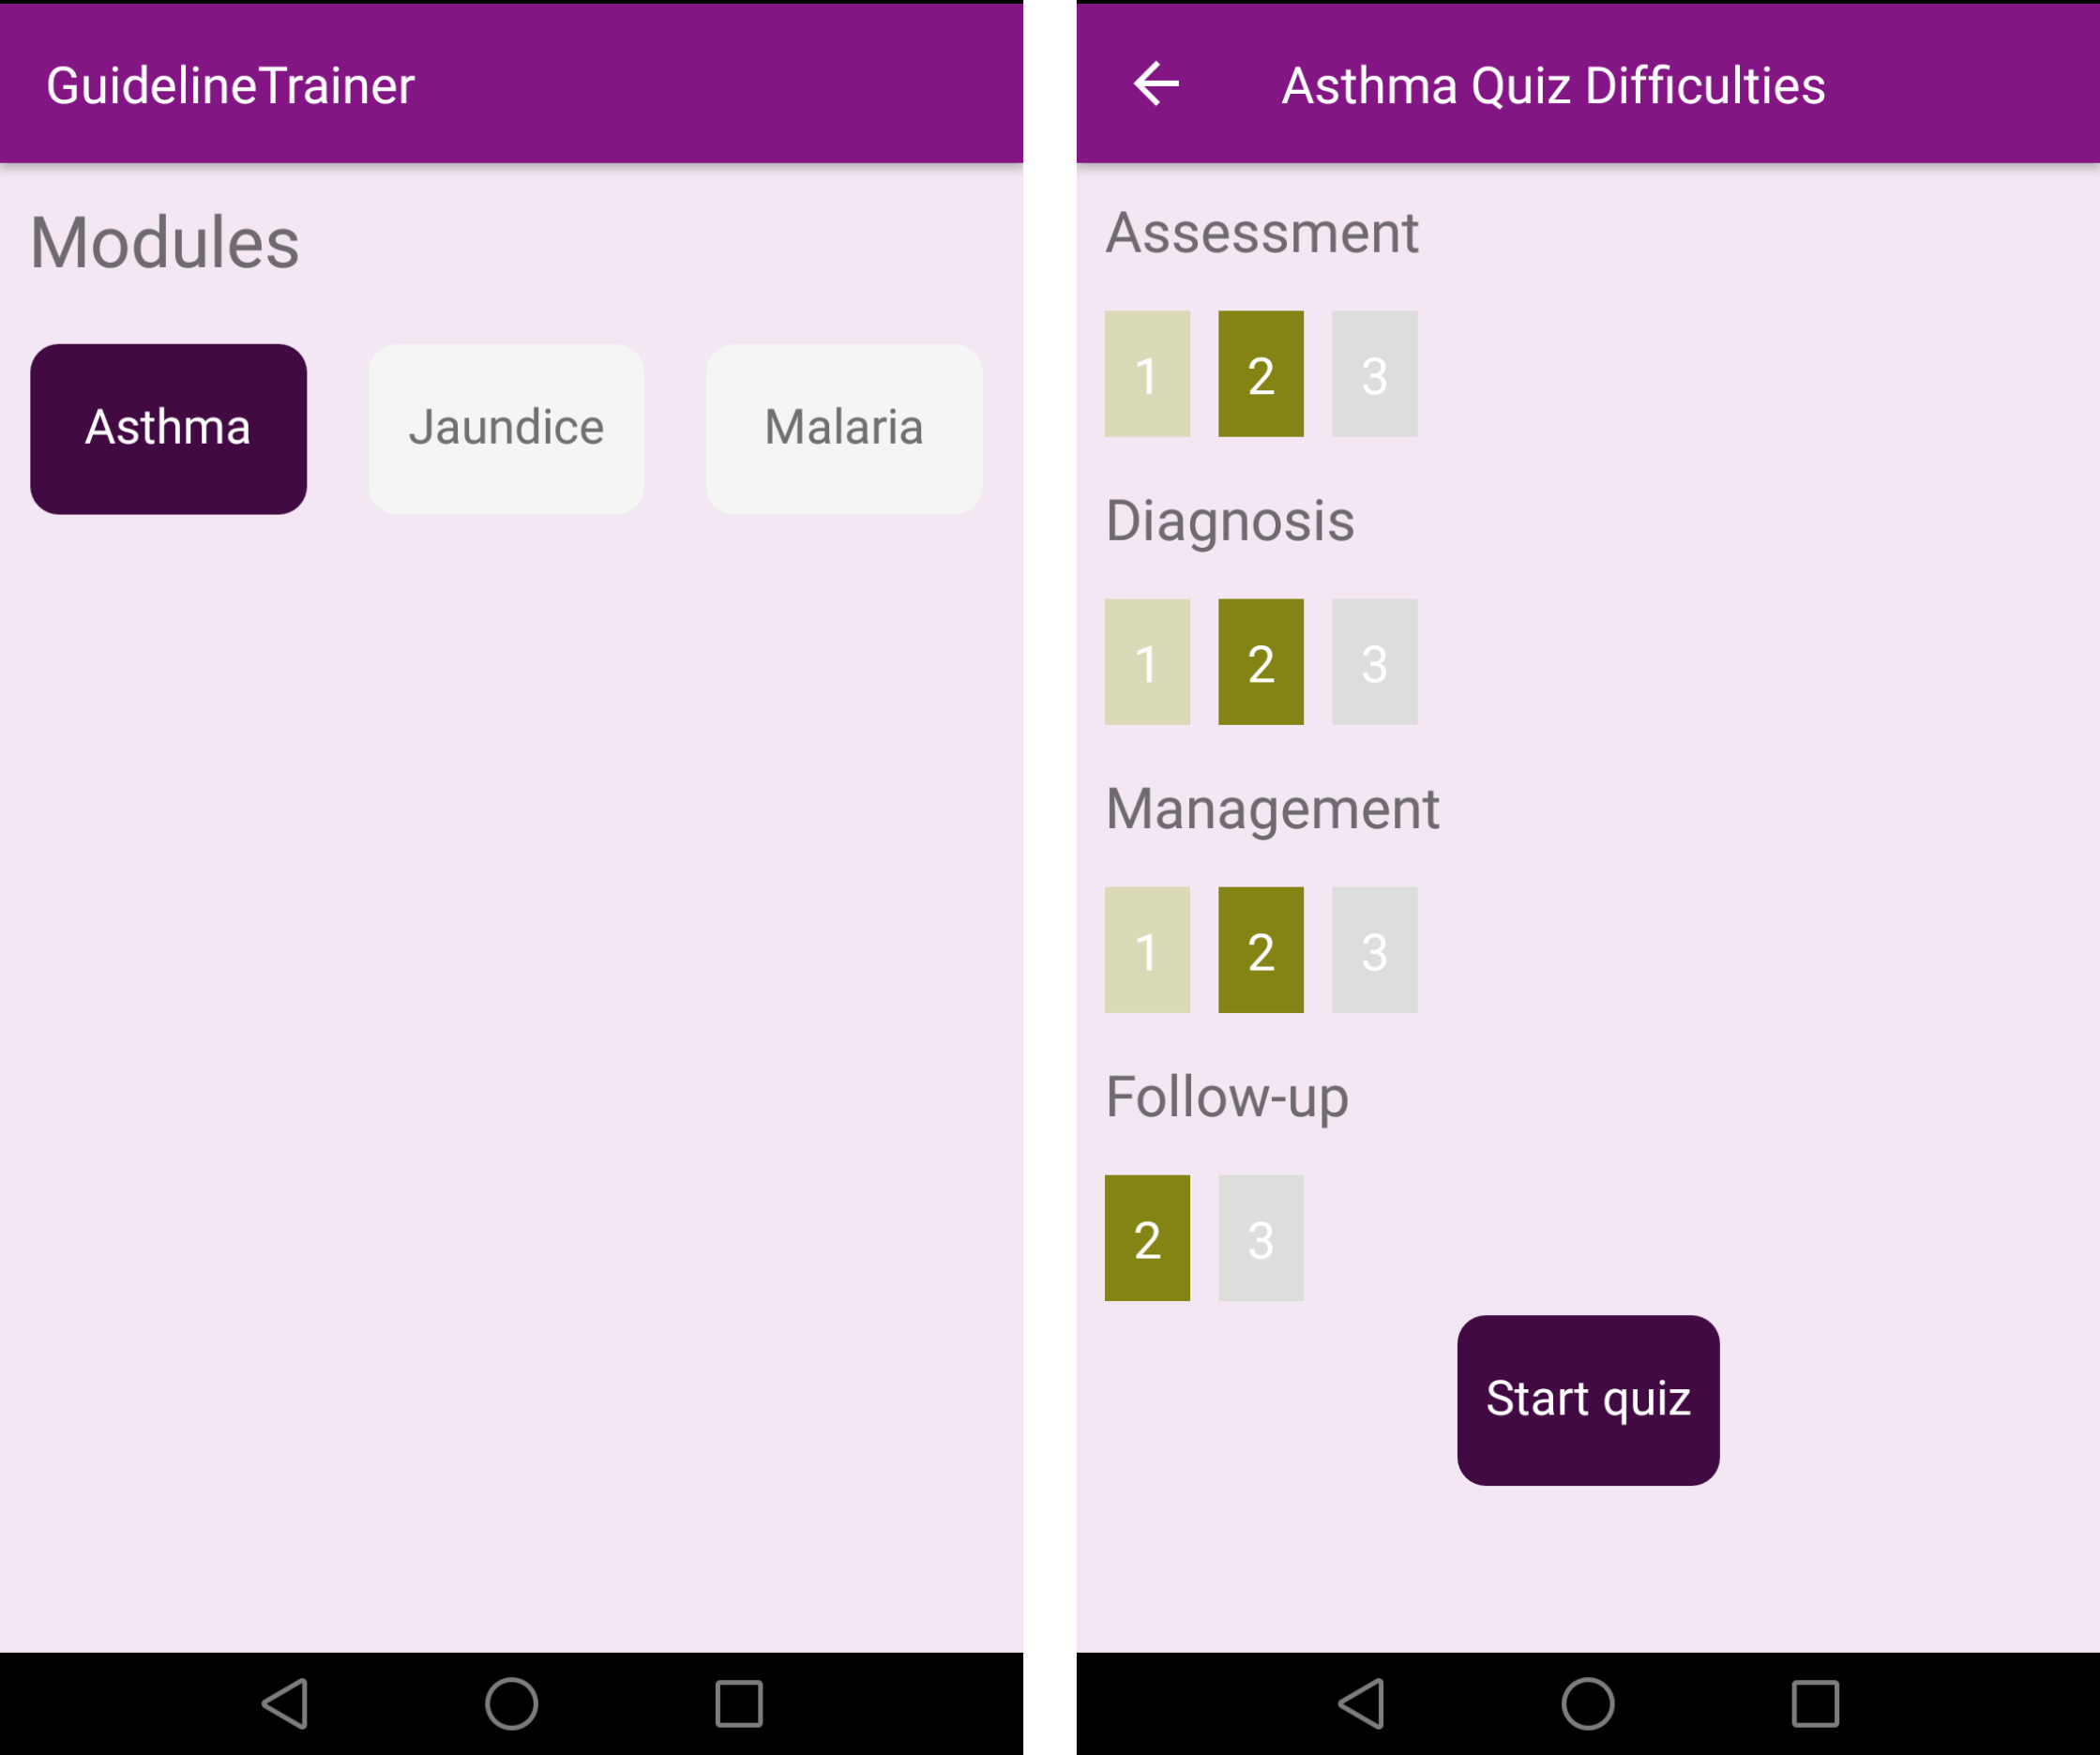
\includegraphics[scale=0.16]{Montage1}
\end{frame}
\begin{frame}{Demonstration}
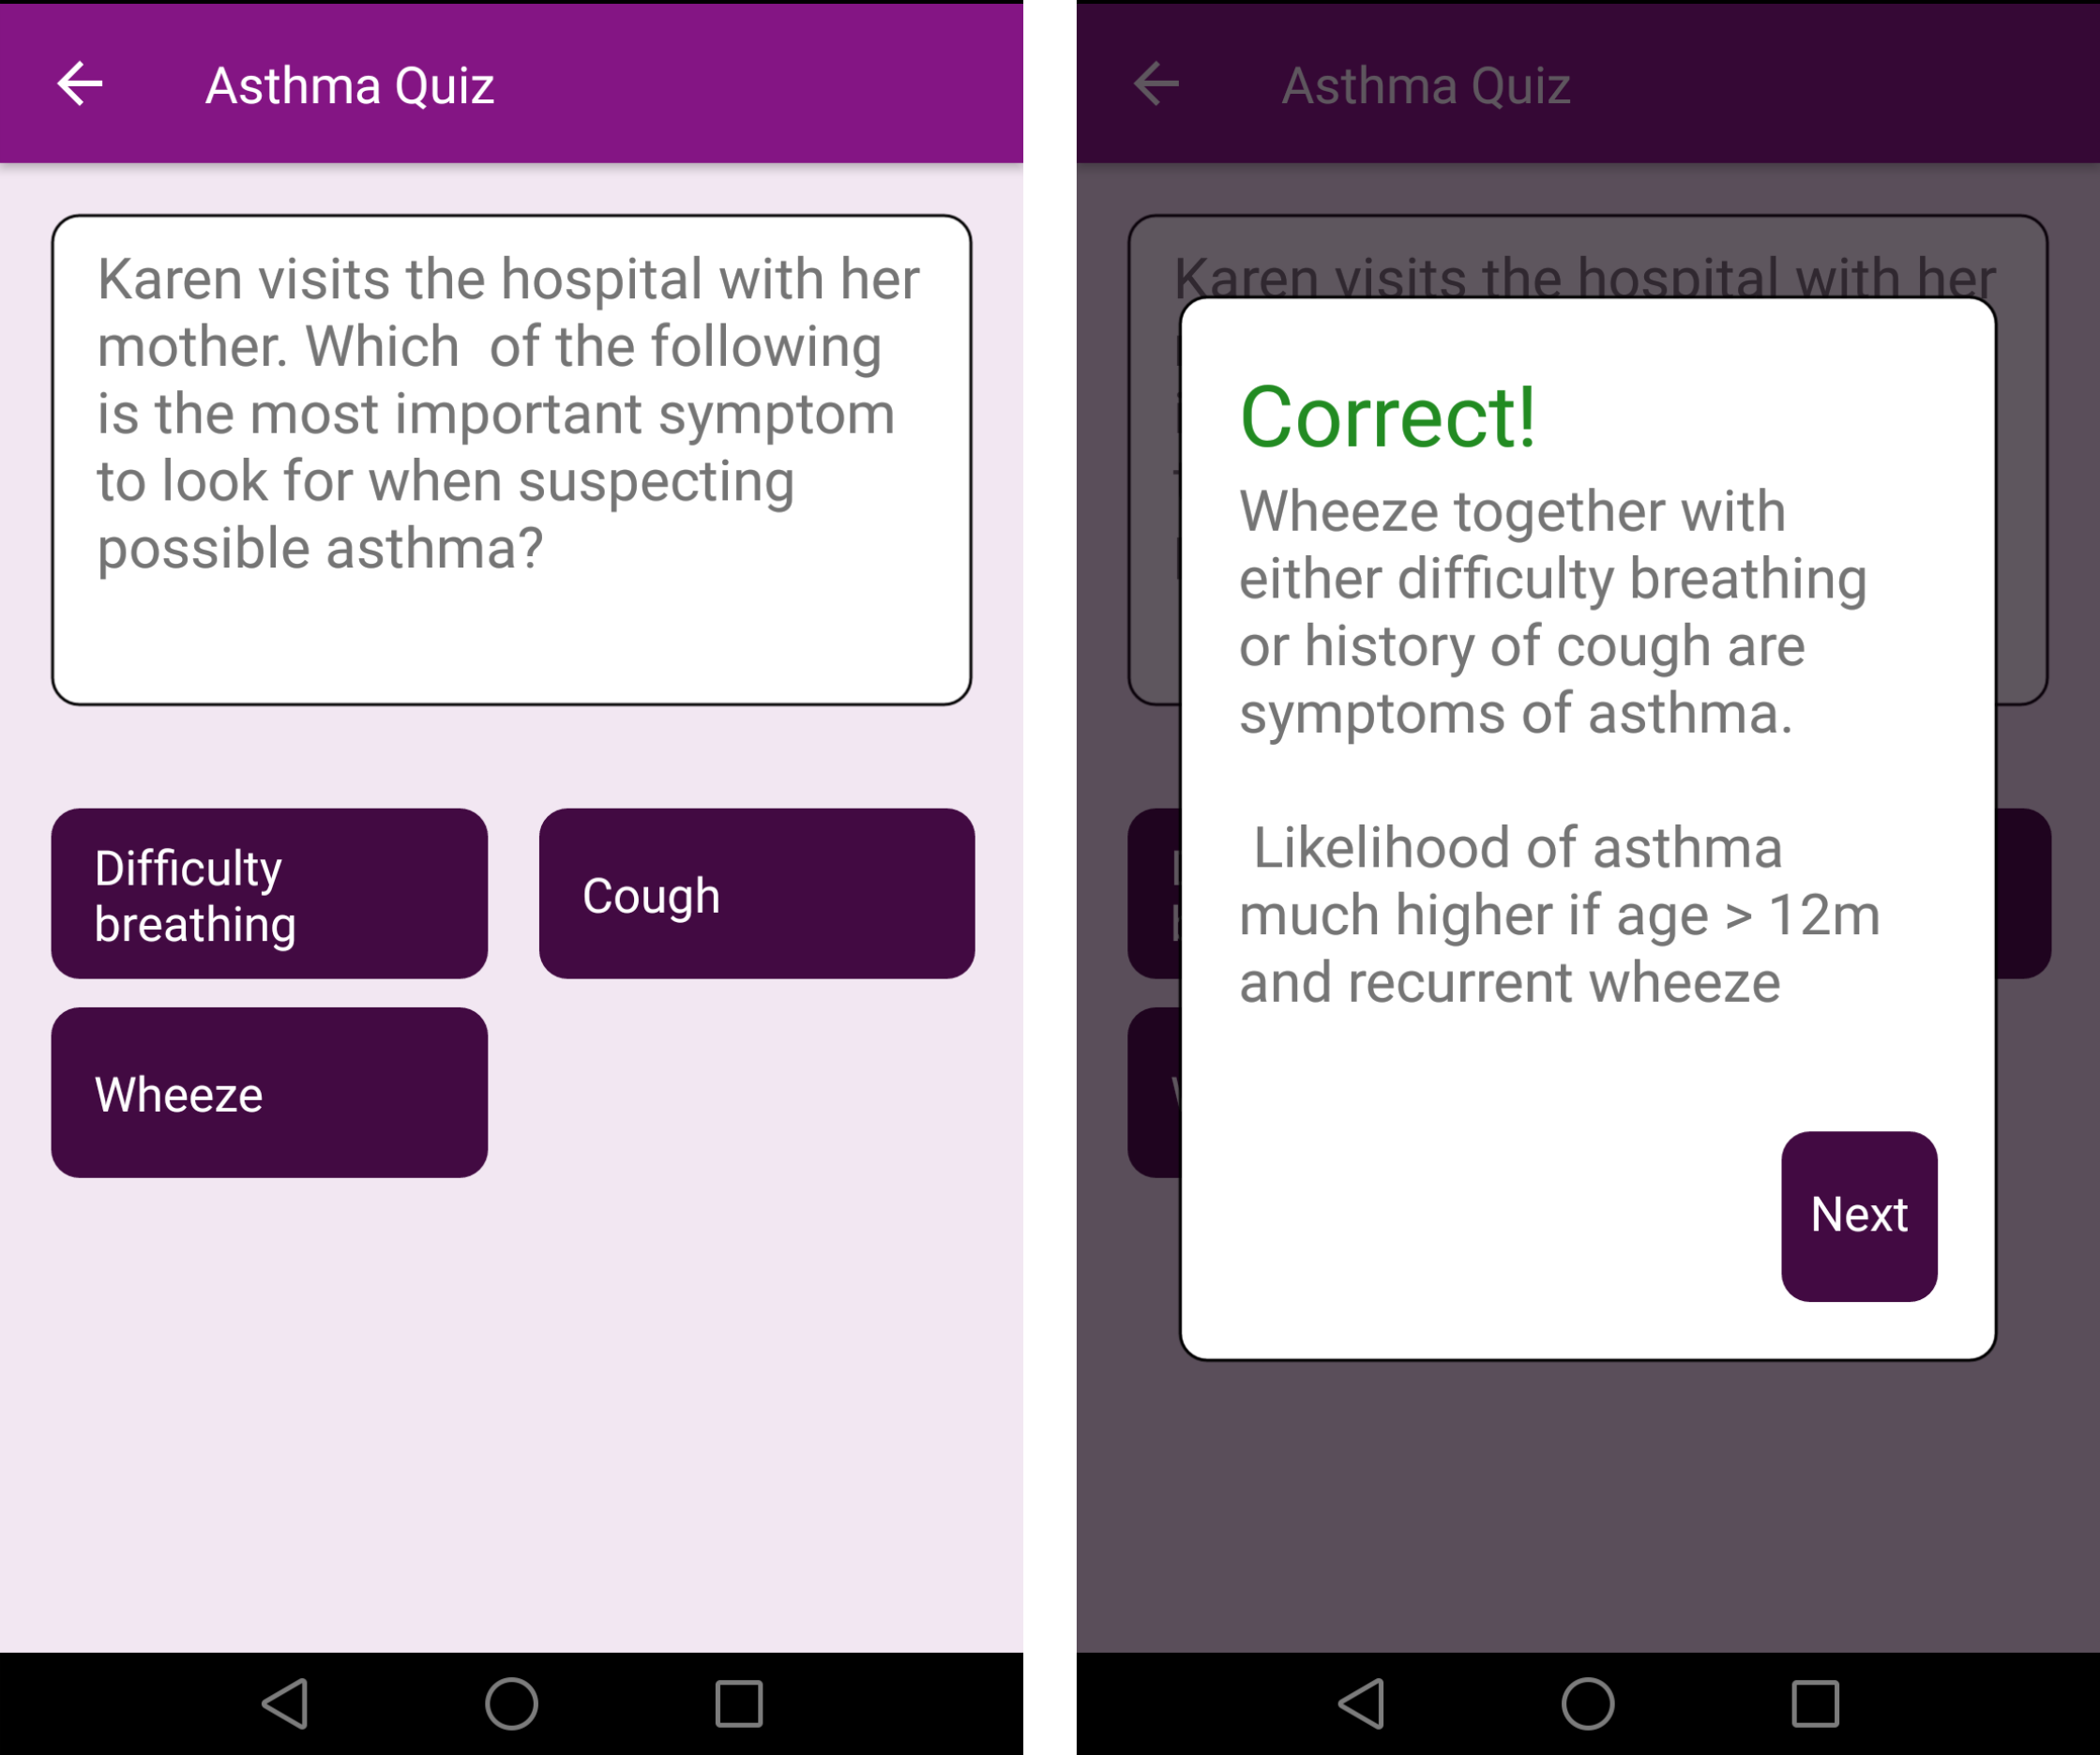
\includegraphics[scale=0.16]{Montage2}
\end{frame}
\begin{frame}{Demonstration}
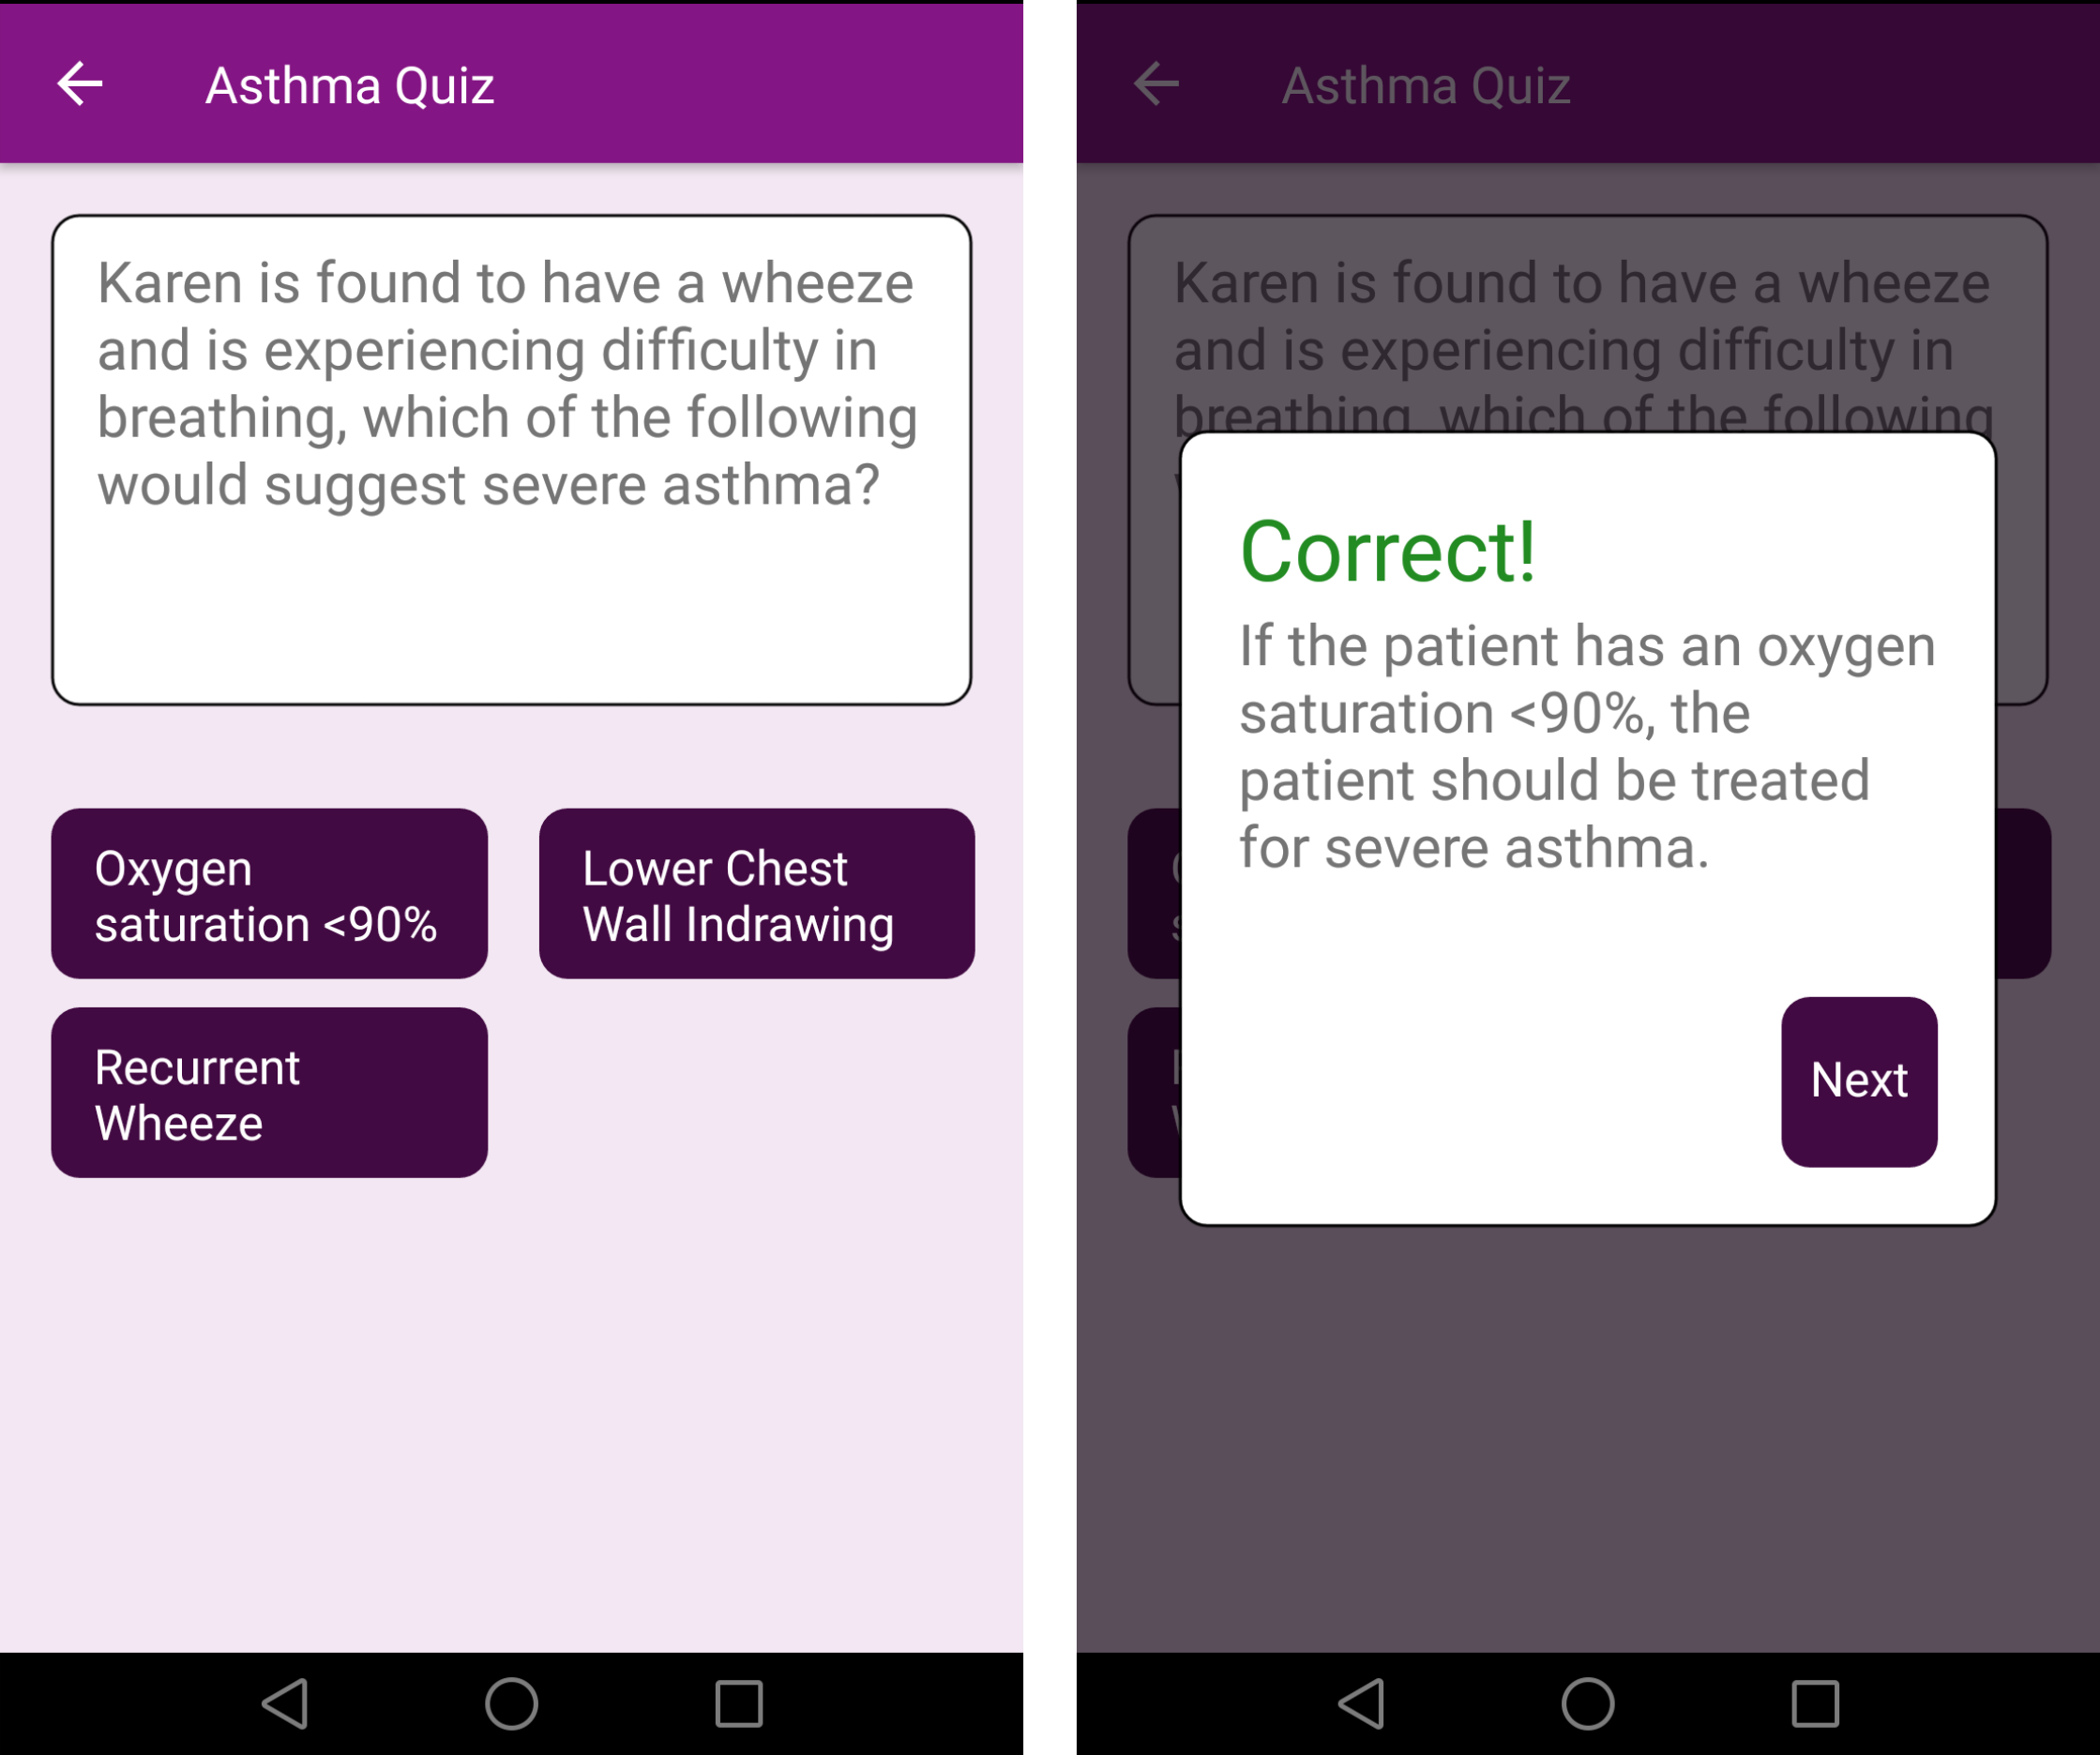
\includegraphics[scale=0.16]{Montage3}
\end{frame}
\begin{frame}{Demonstration}
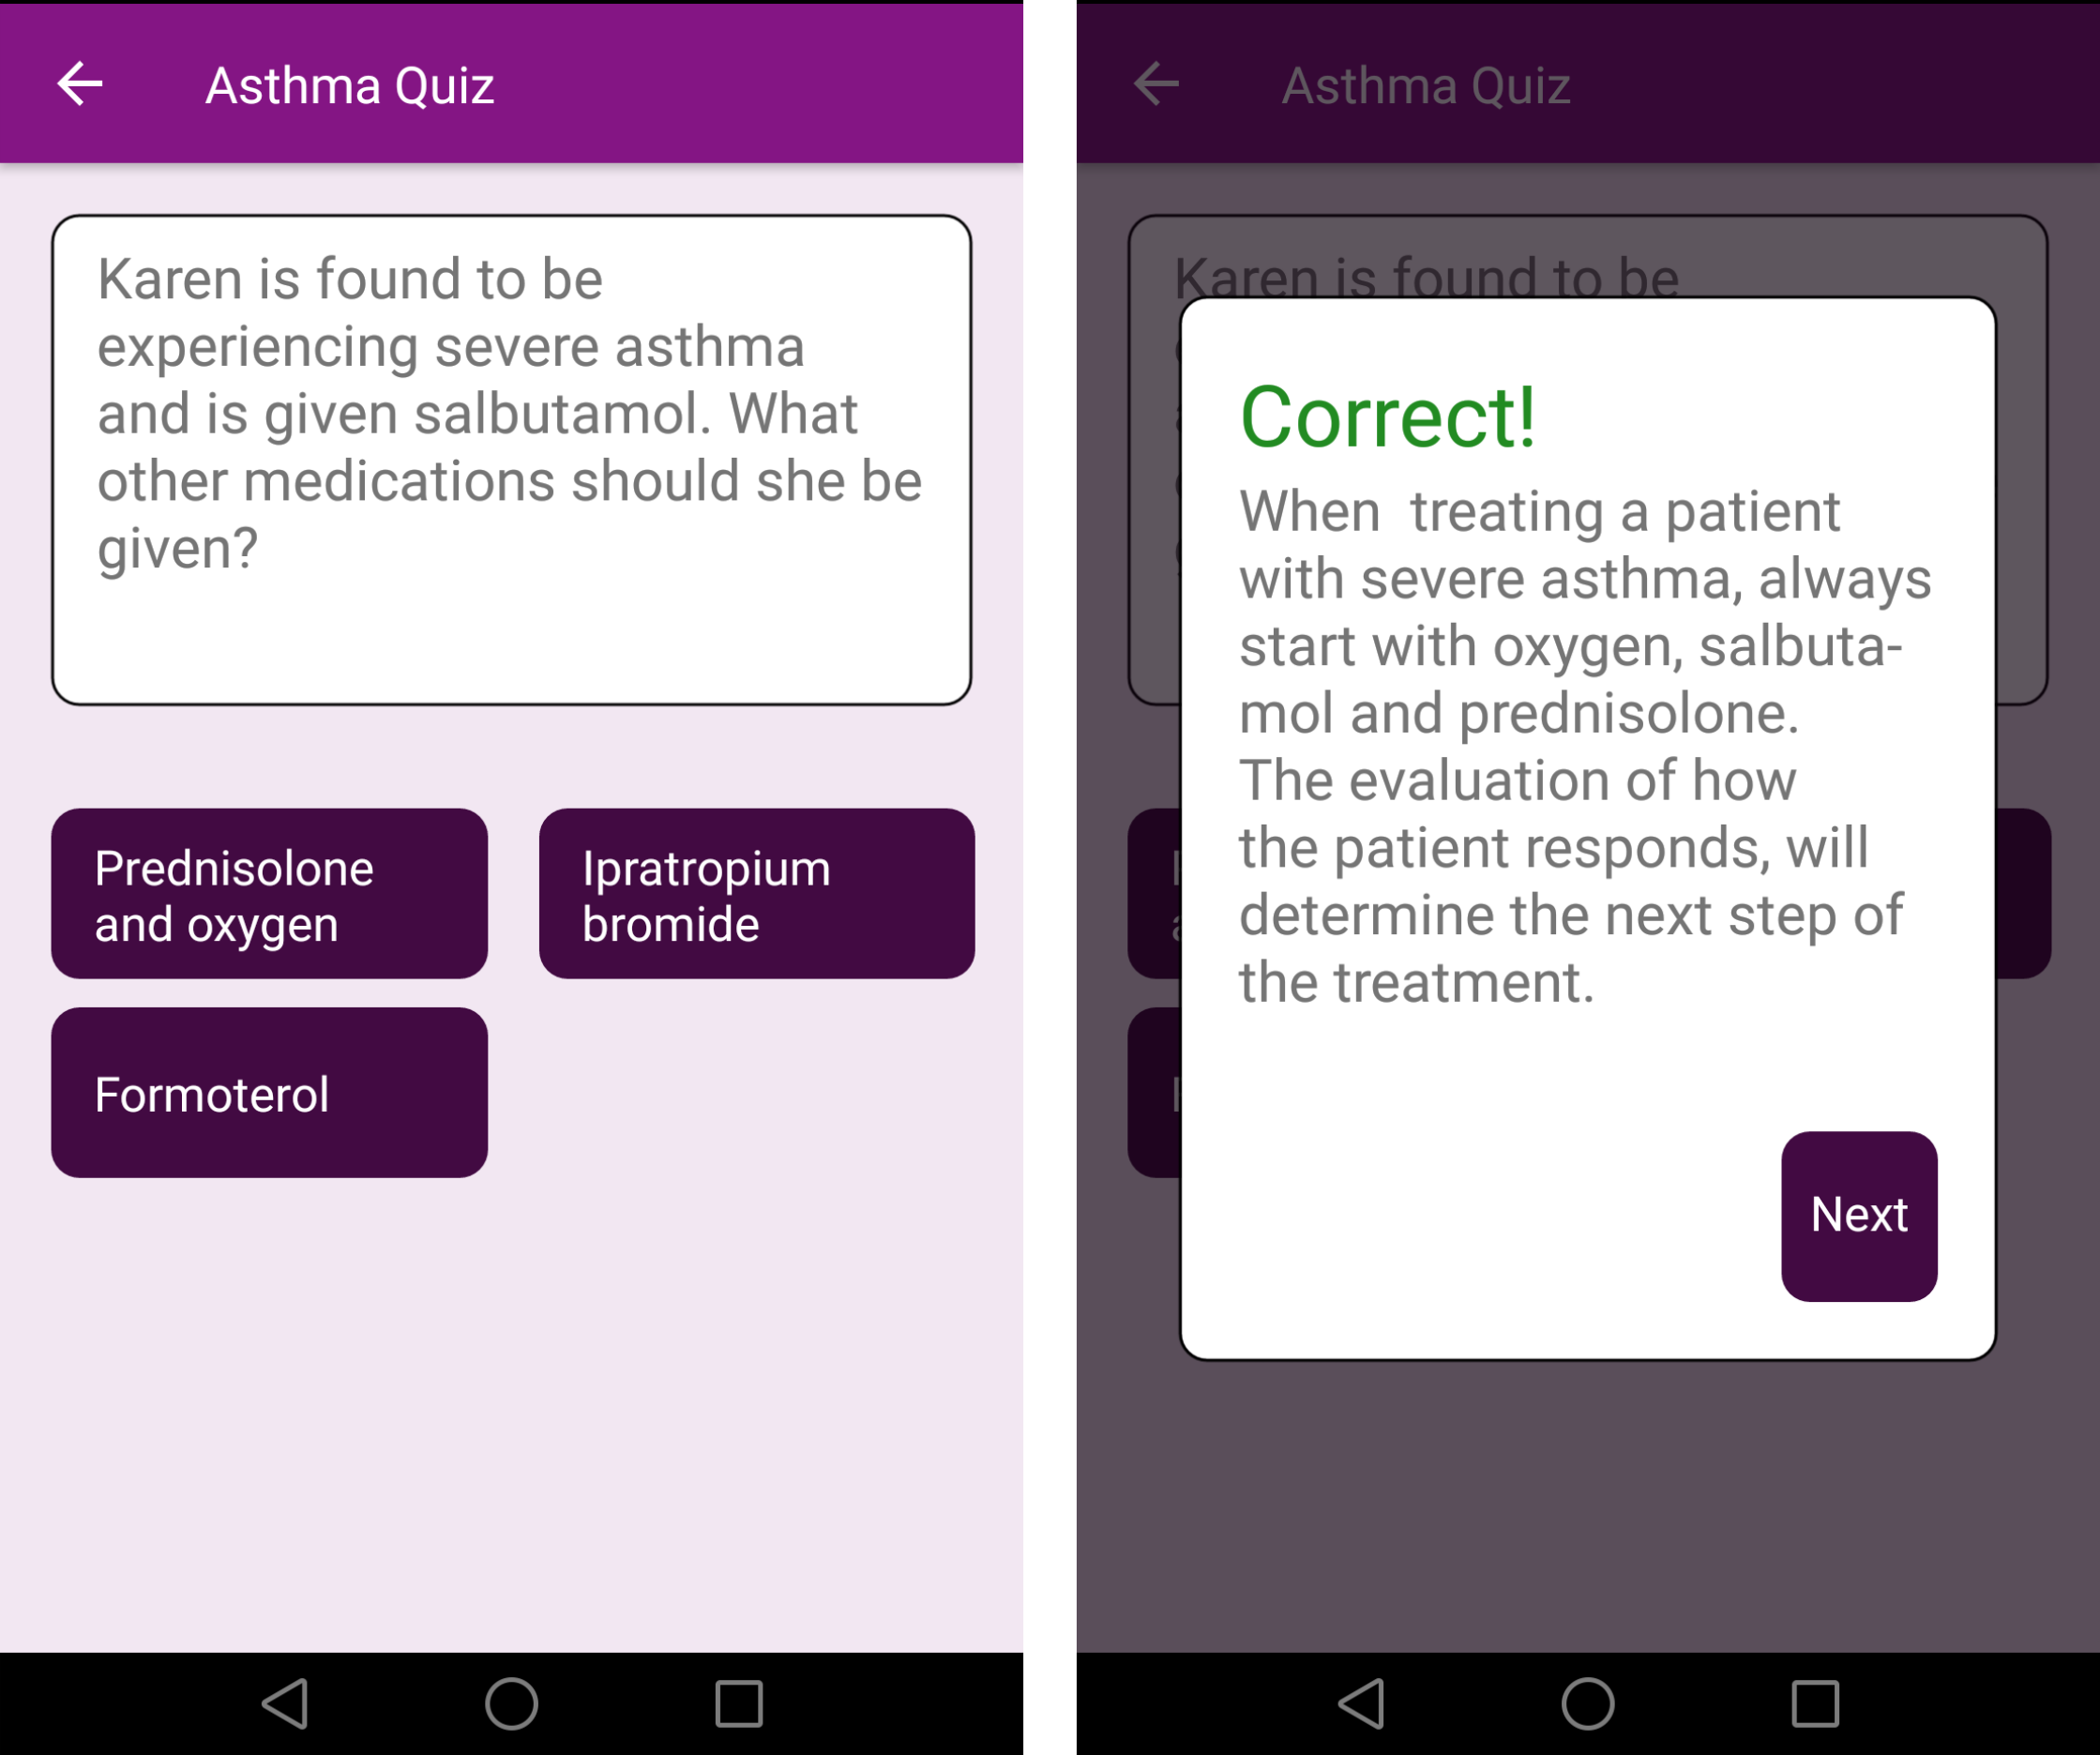
\includegraphics[scale=0.16]{Montage4}
\end{frame}
\begin{frame}{Demonstration}
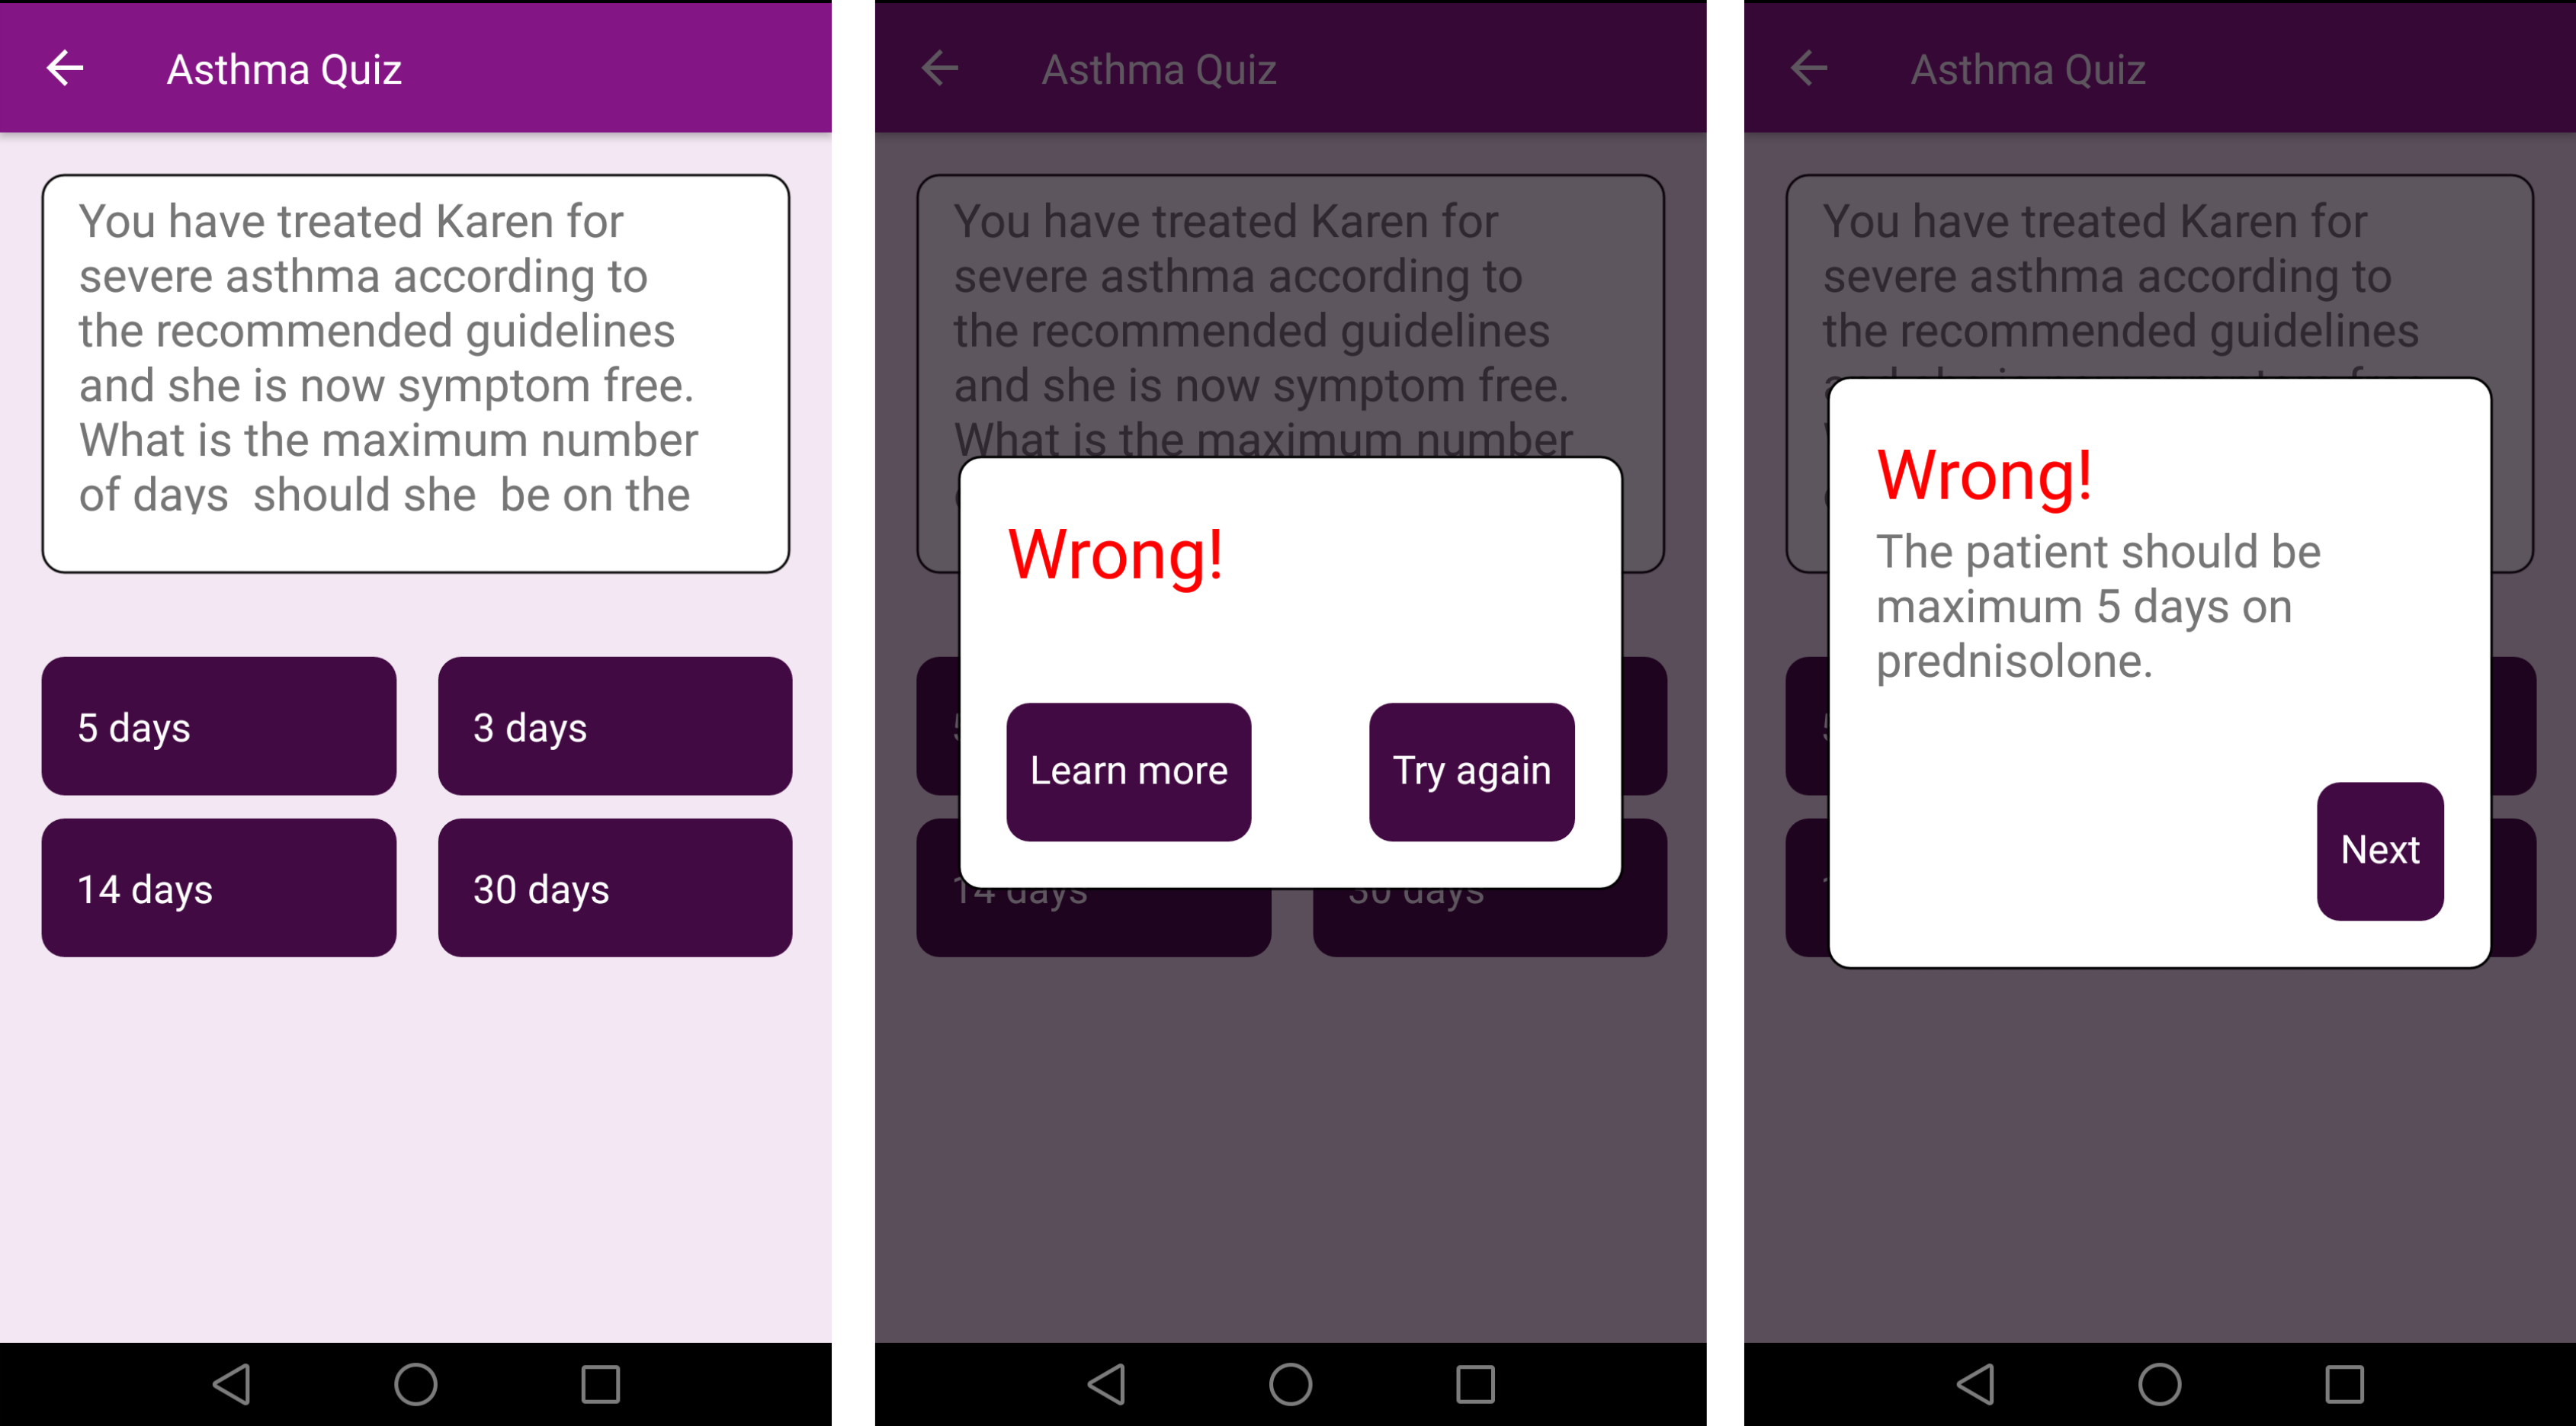
\includegraphics[scale=0.14]{Montage5}
\end{frame}
\begin{frame}{Demonstration}
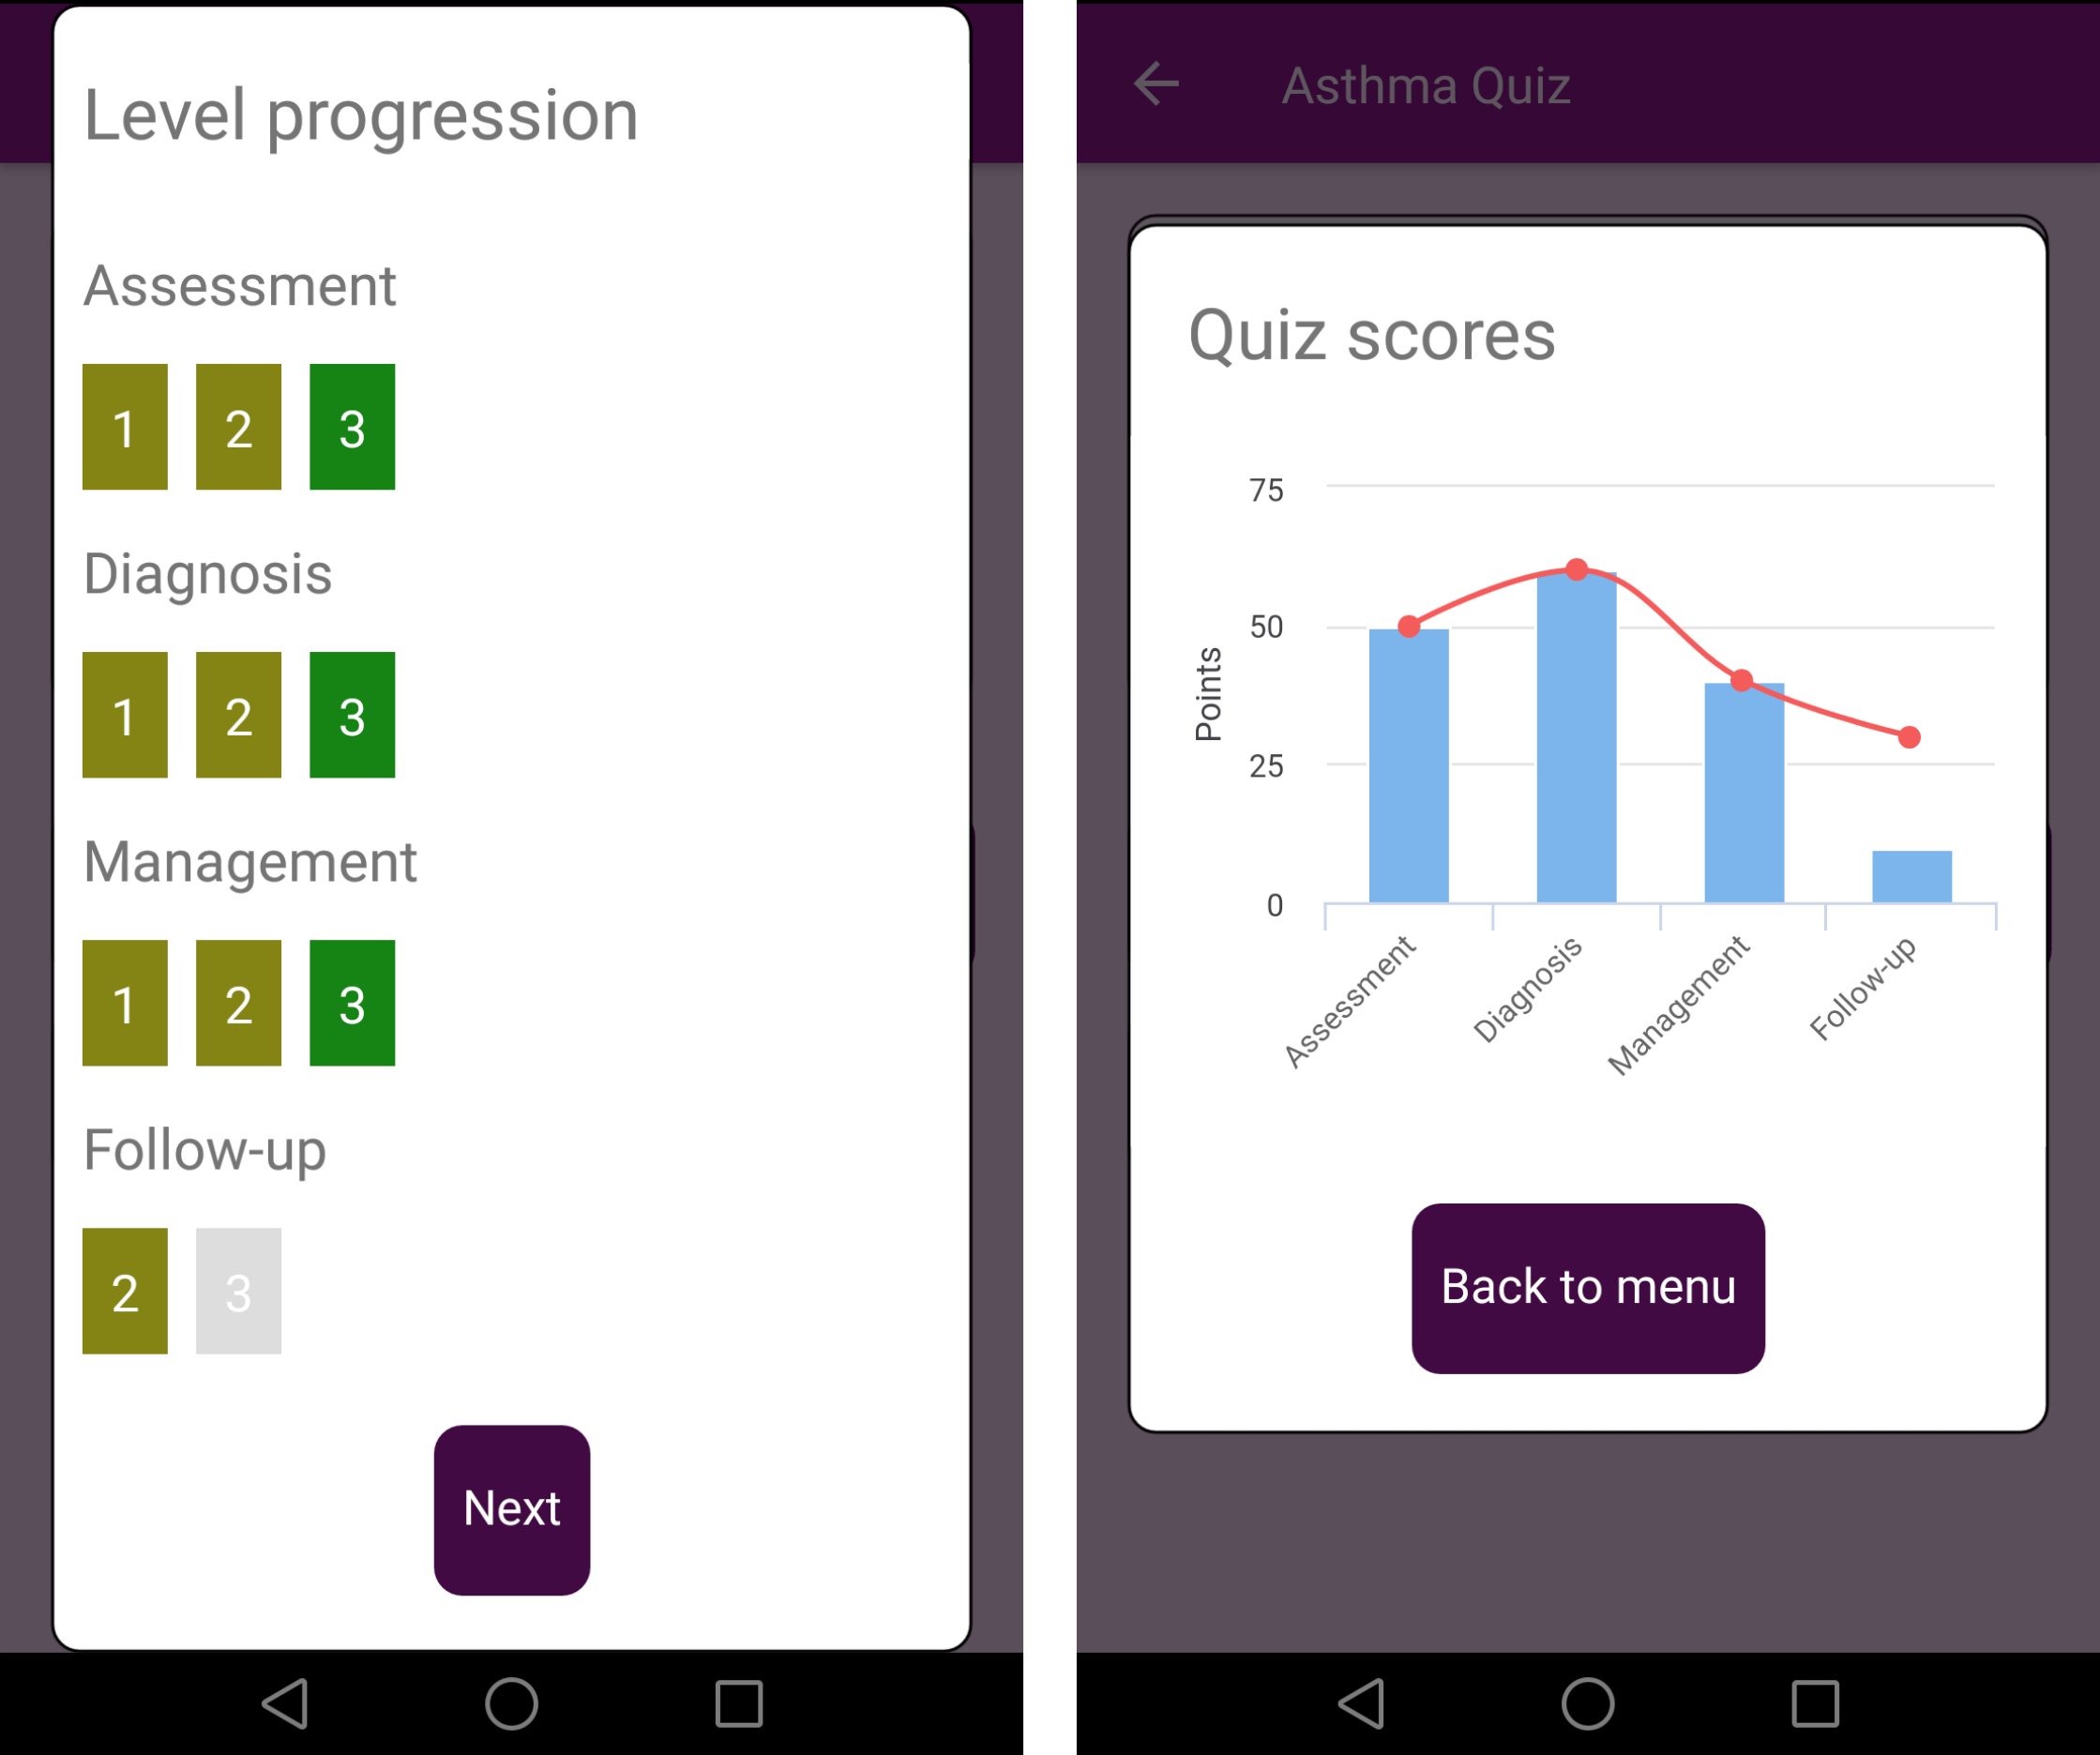
\includegraphics[scale=0.16]{Montage6}
\end{frame}

\begin{frame}{Evaluation}
Planned evaluation
\begin{itemize}
	\item Through user tests, let clinicians or medical students determine the relevance of the artefact.
	\begin{itemize}
		\item Demonstrate how the learning content is adapted to the learners current knowledge level.
	\end{itemize}
	\item Demonstrate that the model can be used to represent other respiratory diseases.
	\item Demonstrate generation of multiple choice questions and answer elements.

\end{itemize}
\end{frame}
\end{document}